\documentclass{article}

\usepackage{graphicx}
\usepackage{amsmath}
\usepackage[margin=1.0in]{geometry}
\linespread{1.5}

\graphicspath{ {images/} } 

\title{A study of heterogeneous materials and wave propagation in phononic
media}
\author{Bryan Chem}
\date{May 14th, 2018}

\begin{document}
\pagenumbering{gobble}

\maketitle
\newpage

\pagenumbering{roman}

\tableofcontents
\newpage

\pagenumbering{arabic}

%----------------------------  INTRODUCTION  ----------------------------------%
%  The purpose of this section here is to introduce the big picture and outline 
%  the rest of the paper. Be sure to do a lot of contextualizing and make 
%  sure the audience knows where you are going.
%------------------------------------------------------------------------------%
\section{Introduction}
Heterogeneous materials appear in all kinds of forms and can be found naturally 
and in industrial applications. Recently, interest has grown in artificially
constructed phononic media which can alter the propagation of acoustic and
elastic waves. A phononic medium is a heterogeneous material which possesses
spatial periodicity in the arrangement of its constituents, its structure,
or the boundary conditions applied to it. As a result of this periodic 
structure, it has been shown that there exists band gaps for which certain 
frequencies of waves cannot propagate. These frequency band gaps have been 
utilized in many engineering applications related to vibrations and the control 
of acoustic and elastic waves.

There were three objectives for this independent study:
\begin{enumerate}
	\item Study heterogeneous materials and the associated mathematical methods 
	used to model their behavior
	\item Study wave propagation in phononic media and the associated 
	computational methods (mainly finite elements)
	\item Complete a computational project related to the above studies 
\end{enumerate}
In this report, the focus will be on the later two items as the study of 
heterogeneous materials was completed via a set of exercises from the lecture 
notes of Prof. Ponte-Casta\~neda \cite{pontenotes}. To this end, phononic media 
and their applications are presented, and the interesting behavior that is the 
presence of frequency band gaps where waves cannot propagate is described. 
After introducing these concepts, the history and state of active research is 
outlined in the literature review section. Dispersion relations and their 
relation to studies in phononic media are introduced and will be central to 
further studies in the report. While it is favorable to have exact analytical 
expressions for these dispersion relations, it is not possible to calculate 
this by hand for more complicated materials. As such we must utilize 
computational methods which are presented in varying levels of detail. For 
future research, it is planned to use the finite element method, and this is 
the computational method that is used in the independent study. Finite elements 
is used in the 1D and 2D case in order to obtain the dispersion relation for a 
variety of materials. These studies will be integral for further research that 
will advance the field.

%----------------------------  PHONONIC MEDIA  --------------------------------%
%  This subsection is dedicatied to illustrating what these materials can do 
%  here you want to get the audience excited about phononic media. What can
%  these things do that regular materials can't make a point of this!
%------------------------------------------------------------------------------%
\subsection{Phononic media}
%  Examples of phononic media
As mentioned before, the field of phononic media has grown tremendously in the 
past two decades and continues to grow today. Examples of phononic media 
include mass spring systems, laminates, and materials embedded with a periodic 
lattice of inclusions (or voids). There are several levels of classification 
within phononic media. In the literature a distinction, is made between 
phononic materials and phononic structures. Phononic materials are infinite in 
extent while phononic structures are finite in extent \cite{hussein10}. 
Phononic crystals refer to a heterogenous material or non-uniform material the 
material phases that may be fluid or solid which have a periodic arrangement in 
space \cite{hussein14}. The constituents may be arranged in such a way as to 
have a band gap in a certain frequency range or may even be tunable such as by 
modulating an outside field the material properties may be changed in order to 
move the band gap. A further class of phononic media that is of much interest 
is the metamaterial. Metamaterials possess ``local resonance" which is a 
different way for producing band gaps that is not seen in phononic crystals. 

%  Applications of phononic media
The existence of frequency band gaps in these materials has resulted in many 
practical applications such as:
\begin{itemize}
	\item \emph{Vibration control}: The simplest application would be to 
	incorporate these phononic media in the construction of buildings or 
	vehicles with band gaps in the range of frequencies of acoustic or elastic 
	waves found in the operating environment in order to provide insulation.
	\item \emph{Acoustic/elastic waveguides}: By simply removing inclusions in 
	a phononic crystal it has been found that wave propagation can be localized 
	to certain areas within the material \cite{hou12}. 
	\item \emph{Acoustic diodes}: It has been found that sonic 
	crystals, which are phononic crystals where one or more of the material 
	phases is a liquid, can be used in 1D acoustic diodes which allow certain 
	waves to propagate in one direction but not in the opposite direction 
	\cite{zhang10}.
	%  I need to read more on these last two
	\item \emph{Subwavelength imaging}:
	\item \emph{Cloaking}:
\end{itemize}
This, of course, is a non-exhaustive list with new studies in materials with 
tunable properties, damping, non-linear affects, and disorder other novel and 
useful applications will arise.

%------------------------------  BAND GAPS  -----------------------------------%
%  Why can these phononic media do what they do? We are still not talking about
%  anything that you have done yet. Setting the stage still.
%------------------------------------------------------------------------------%
\subsection{Band gaps}
All of the above applications rely on presence of band gaps in these phononic 
media. There are two mechanisms which cause band gaps to form:
\begin{enumerate}
	\item \emph{Bragg scattering}: At certain frequencies, waves can interact 
	with the structure of a material in such a way that reflections off of 
	inclusions or the structure of material itself destructively interfere with 
	the incident wave. Here, the behavior is dependent on the periodicity in 
	the arrangement of the material phases or structure of the material 
	\cite{laude15}.
	\item \emph{Local resonance}: When resonators are placed inside of a 
	materials, interactions occur at the resonant frequency of the resonator. 
	At these frequencies, the resonators begin to absorb energy from incident 
	waves and produce a band gap.
\end{enumerate}
These two mechanisms have predictable effects on the frequency band structure 
of phononic media. 

%  I thought I just read in hussein that bragg scattering for low frequencies 
%requires larger spacing ... etc.

%---------------------------  LITERATURE REVIEW   -----------------------------%
%  You have told the audience about phononic crystals and why they are special.
%  Now it is time to contextualize this field of research and get them excited 
%  about not just the special properties, but the plethora of research 
%  oppurtunities still available in this field. Even before the histor and 
%  active fields, I would start by motivating the theoretical research like 
%  Hussein does. Read that section again.
%------------------------------------------------------------------------------%
\section{Literature review}

%------------------------  HISTORY OF PHONONIC MEDIA   ------------------------%
%  You don't need to be too verbose here. Yes, include when these materials 
%  first studied in order to show how young the field is. Really, this is the 
% part where you show what has been done. You have to know what has been 
%  done before you do anything.
%------------------------------------------------------------------------------%
\subsection{History of phononic media}

%----------------- ACTIVE REASEARCH AREAS AND OPEN FIELDS    ------------------%
%  This is where you need to be verbose. Show the audience you know where this
%  field of research is today and your place in it. Inculde plenty of references
%------------------------------------------------------------------------------%
\subsection{Active research areas and open fields}

%---------------------------------  DAMPING   ---------------------------------%
%  You have many good references here but only from Hussein and Frazier. Try to 
%%%  include references from two other authors. Damping is pretty easy to write 
%%%%  about
%------------------------------------------------------------------------------%
\subsubsection{Damping}
In applications, energy is often lost through damping. This will affect the 
propagation of waves, and thus models that consider this effect will better 
represent the actual behavior of a material. Within the body of research on 
damping, studies focus on either harmonic wave propagation or free wave 
propagation. A study of harmonic wave propagation entails one in which the wave 
numbers are confined to be real while free wave propagation allows for complex 
wave numbers (and as a result evanescent waves). Standard computational methods 
as discussed in Section \ref{methods} are used in both types of studies. 

In \cite{hussein14}, dispersion relations are first obtained for a 1D diatomic 
lattice with linear viscous damping. The method of analysis for this example is 
then extended to a 1D lattice with internal resonators and also a 2D phononic 
crystal with square unit cells embedded with a single, denser square inclusion. 
The general result of including damping is the collapase of the band gap 
between the optical and acoustic branches of the dispersion relation. This 
occurs such that the optical branch lowers proportional to the amount of 
damping.

%----------------------------- NONLINEAR SYSTEMS ------------------------------%
%  Same thing here. You will need to branch out in terms of references here.
%------------------------------------------------------------------------------%
\subsubsection{Nonlinear systems}
Relative to linear studies, there have been fewer studies of nonlinear phononic 
materials. Due to nonlinearities, Bloch's theorem cannot not be applied in the 
same way to obtain an eigenvalue problem for the dispersion relation -at least 
not immediately. Perturbation techniques have been developed as early as 1994 
in order to study weakly non-linear systems. These techniques ``expand" the 
governing equations and produce a linear equation while instead considering the 
nonlinearities to be a part of forcing term.

%-------------------------- DISORDERED MATERIALS ------------------------------%
%  This is also an easy one to write about. The challenges and the reason why
%  there are so few references is obvious.
%------------------------------------------------------------------------------%
\subsubsection{Disordered materials}
Just as sparse as nonlinear systems, the study of phononic media with disorder 
has not been widely researched. Incorporating even small amounts of disorder 
can increase the predictablility of a model much like damping. In the 
manufacturing process perfect periodicity may not be able to be acheived. The 
difficulty in disordered phononic media is that the conventional method of 
Bloch wave analysis does not work. A requirement of Floquet-Bloch theory is 
that the material properties vary periodically with a known period. A single 
unit cell can no longer model the behavior of the entire system if there is 
even mild disorder.

Recently, there has been research done on so called hyperuniform phononic 
crystals. Hyperuniformity is a way of categorizing point distributions. It 
specifically refers to distributions with the fluctuations in density completly 
vanish as the window of observation increases. Despite not having any 
periodicity, and therefore no Bragg peaks, there still exists band gaps.

An earlier paper in 2010 by, examined a 2d phononic medium with circular 
inclusions arranged in a lattice. Disorder was added to the system by 
increasing or decreasing the size of the inclusions or displacing them by some 
small amount. Here they used the plane-wave expansion method. Of course, due to 
the added disorder they were no longer able to look at a single unit cell and 
instead define a `supercell' for which the analysis was carried out. 


%--------------------- DYANMIC EFFECTIVE PROPERTIES  --------------------------%
%  Tie this into homogenzation. Remember this is a part of your independent 
%  study and you should have some insight here.
%------------------------------------------------------------------------------%
\subsubsection{Dynamic effective properties}
With any heterogeneous material, it is of interest to be able to define 
effective properties and model the material as one homogenous material. This 
reduces the computational cost of modeling. Most analysis in homogenization has 
been done in the long wavelength limit. Trying to perform a similar type of 
analysis on a material with dispersive properties results in the loss of this 
behavior. The problem here lies in the volume averages used to calculate the 
effective properties. The richness in behavior of these phononic media is due 
to the relative motion of contituents as such the behavior is said to be 
nonlocal and this must be taken into affect when trying to formulate dynamic 
effective properties.

Michael Frazier has done some work calculating the dynamic effective viscosity 
in damped 1D layered structures.

%--------------------------- DISPERSION RELATIONS  ----------------------------%
%  Okay so now you've been doing a lot of talking about past and current 
%  research. You absolutely cannot just jump into dispersion relations. This is
%  going to need some good framing. i.e. to do research we need to know about
%  this. This section needs to highlight the importance of dispersion relation
%  and just how much information is jam packed into this little thing
%------------------------------------------------------------------------------%
\section{Dispersion relations}
Dispersion relations provide all of the information necessary to characterize 
the behavior of waves propagating in a phononic medium. Mathematically, they 
are a relationship between the frequency of a wave and its wavenumber. From 
this relationship, it is possible to determine the phase velocity and group 
velocity. Dispersion relationships immediately indicate where the frequency 
band gaps of a system are. For this reason, they are also called frequency band 
diagrams or frequency band structures.

As will be shown, there are a variety of waves to calculate dispersion 
relations, however, there is a commonality between each type of analysis. This 
common feature is the application of Floquet-Bloch theory.

%-------------------------- FLOQUET-BLOCH THEOREM  ----------------------------%
%  To derive dispersion relations you need to know this theorm. It is an 
%  important result and should not be presented without proof. Important to
%  maintain a connection with dispersion relations and phononic media here.
%------------------------------------------------------------------------------%
\subsection{Floquet-Bloch theorem} \label{fbt}
Given the equation
\begin{equation} \label{floqueteqn}
\frac{\partial^2 u}{\partial x^2} + c(x)y = 0
\end{equation}
where \underline{c(x) is periodic in} $x$, Floquet's theorem says that 
(\ref{floqueteqn}) has two solutions
\begin{align*}
u(x) &= \tilde{u}_1(x)e^{ikx} \\
&= \tilde{u}_2(x)e^{-ikx}
\end{align*}
In the above, $\tilde{f}_1$ and $\tilde{f}_2$ are also periodic in $x$ 
\cite{magnus79}.

Bloch's theorem is similar to Floquet's theorem but applies to higher 
dimensions \cite{laude15}. 

Given
\begin{equation} \label{blocheqn}
-\nabla \cdot \left( c(\mathbf{r}) \nabla u(\mathbf{r}) \right) = \omega^2 
u(\mathbf{r})
\end{equation}
where \underline{$c(\mathbf{r})$ is periodic in space}, Bloch's theorem says 
equation (\ref{blocheqn}) has eigensolutions
\begin{equation}
u(\mathbf{r}) = \tilde{u}(\mathbf{r}) e^{-i\mathbf{k} \cdot \mathbf{r}} 
\end{equation}
These eigensolutions are called \emph{Bloch waves} and equation 
(\ref{blocheqn}) is called the periodic Helmholtz equation.

%-------------------- FIRST PRINCIPLES AND EXAMPLE PROBLEMS -------------------%
%  Here we dive into more technical analysis. The audience is introduced to 
%  dispersion relations mathematically and also phase and group velocities. Also
%  Introduced is the inverse and direct method. Still want to stay connected,
%  but don't need to try too hard as long as you have done a good job of 
%  framing earlier
%------------------------------------------------------------------------------%
\subsection{First principles and example problems}

\subsubsection{Scalar wave equation}
The scalar wave equation is 
\begin{equation} \label{swe}
\frac{\partial^2 u}{\partial t^2} = c^2 \frac{\partial^2 u}{\partial x^2}
\end{equation}
where $u$ is the displacement and $c$ is the wave speed. Assume a solution of 
the form
\begin{equation}
u(x,t) = A\sin(kx - \omega t)
\end{equation}
In fact, we can assume $u(x,t) = f(kx-\omega t)$ and the following results will 
still hold. $k$ is the wave number which describes the ``spatial" frequency of 
the wave for a fixed time and $\omega$ is the angular frequency that describes 
the temporal frequency of the wave. Substituting this solution into the wave 
equation gives
\begin{equation}
\omega^2 = c^2 k^2
\end{equation}
Taking the square root of the above
\begin{equation} \label{nd}
\omega = \pm c k
\end{equation}
This equation gives a relationship between the frequency of the wave and its 
wave number. We call relations of this type dispersion relations. In general, 
dispersion relations can be written in the form
\begin{equation} \label{wk}
\omega = \omega(k)
\end{equation}
To get a flavor for what dispersion entails, we need to look at the phase 
velocities waves. The phase velocity of a wave is
\begin{equation}
v_p = \frac{\omega}{k}
\end{equation}
Thus, for the scalar wave equation discussed in this introductory paragraph
\begin{equation}
v_p = c
\end{equation}
This relation holds for all waves admissible according to (\ref{swe}). Here, 
every wave propagates at the same velocity regardless of frequency. In this 
case, we say that there is \underline{no} dispersion. In systems with 
dispersion we expect a relation in the form (\ref{wk}) and also
\begin{equation}
v_p = v_p(\omega) = v_p(\omega(k))
\end{equation}

\subsubsection{Monatomic lattice} \label{monatomic}
Take a system of $n$ masses and springs like in Figure \ref{fig:ms} 
\begin{figure}[!htbp]
	\centering
	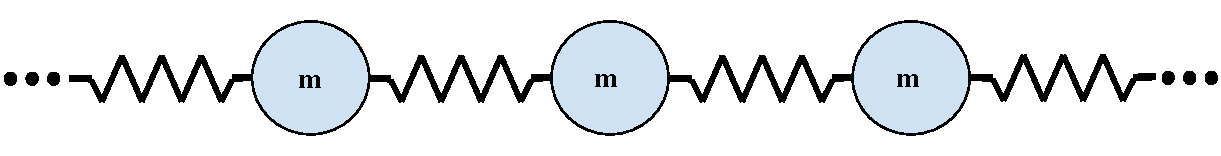
\includegraphics[width=0.75\textwidth]{mass-spring.pdf}
	\caption{A system of masses connected by springs extending infinitely to 
	the left and right.}
	\label{fig:ms}
\end{figure}
Lets write the equations of motion for the $n$th mass system.
\begin{equation} \label{eqnms}
m\frac{\partial^2 u_n}{\partial t^2} = k(u_{n-1} - u_n) - k(u_n - u_{n+1}) = 
ku_{n-1} - 2ku_n + ku_{n+1} 
\end{equation}
where $u_n$ gives the displacement of the $n$th node and $k$ is the spring 
constant of each spring. To acquire, the dispersion relation for this system we 
assume a solution of the form
\begin{equation} \label{bloch}
u_n = Ae^{i(kx_n-\omega t)}
\end{equation}
$A$ is the amplitude of the wave and $x_n = nl$ where $l$ is the distance 
between the masses. Substituting the above into the equation of motion
\begin{align*}
-m \omega^2 u_n   &= ke^{i(k(n-1)l - \omega t)} - 2ku_n + ke^{i(k(n+1)l - 
\omega t)} \\
&= ke^{-ikl}u_n + ke^{ikl}u_n - 2ku_n \\
&= k\cos(kl)u_n - 2ku_n
\end{align*}
Thus,
\begin{equation}
\left[2\omega_0^2(1 - \cos(kl)) - \omega^2\right]u_n = 0
\end{equation}
where $\omega_0 = \sqrt{k/m}$ The above has a trivial solution when $u_n = 0$. 
Not so trivial solutions exist when
\begin{equation}
2\omega_0^2(1 - \cos(kl)) - \omega^2= 0
\end{equation}
We can write the dispersion relation for waves propagating through our mass 
spring system as
\begin{equation} \label{monatomicdisp}
\omega = \pm \sqrt{2\omega_0^2(1 - \cos(kl))}
\end{equation}
It is now becoming apparent that in a system of $n$ masses and springs that 
there is dispersion. To see this explicitly, write the phase velocity
\begin{equation}
v_p = \frac{w(k)}{k} = \frac{\pm\sqrt{2\omega_0^2(1 - \cos(kl))}}{k}
\end{equation}
Clearly, the phase velocity is a function of wave number/frequency which 
indicates dispersivity of the system.

Take our dispersion relation (\ref{monatomicdisp}) and nondimensionalize by 
letting $\Omega=\frac{\omega}{\omega_0}$ and $\mu=kl$. Then,
\begin{equation}
\Omega = \pm \sqrt{2(1-cos(\mu))}
\end{equation}
The positive part is plotted in Figure \ref{fig:dr}.
\begin{figure}[!htbp]
	\centering
	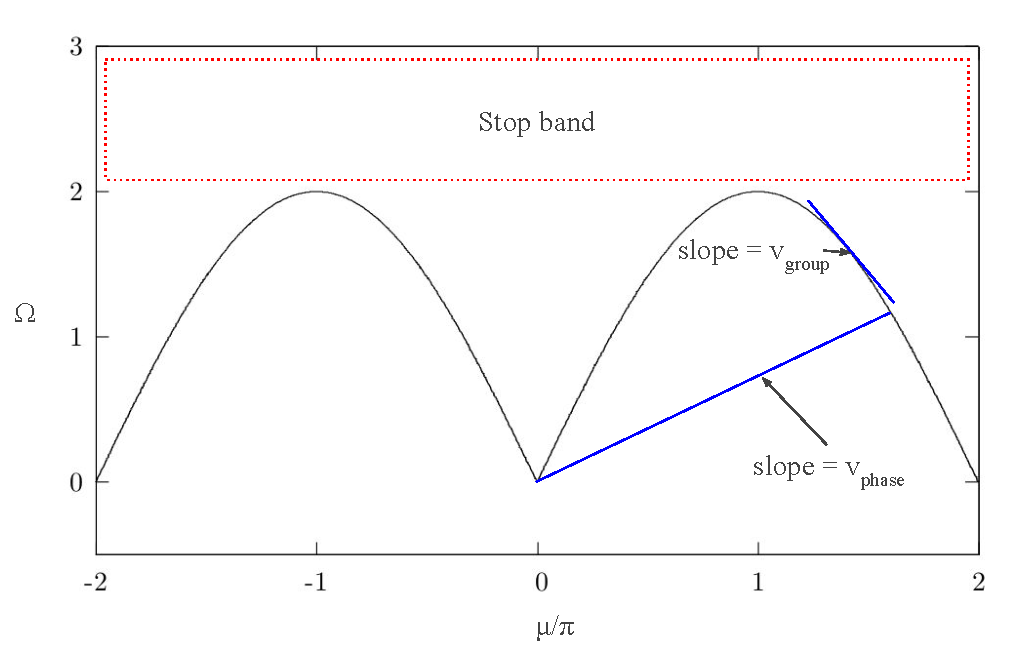
\includegraphics[width=0.75\textwidth]{dispersion-rln.pdf}
	\caption{The non-dimensional dispersion relation for the mass spring system}
	\label{fig:dr}
\end{figure}
The dispersion relation characterizes many features of the mass-spring system. 
In Figure \ref{fig:dr}, it is easy to identify the phase and group velocities 
along the curve for different waves propagating through the system. 

At first glance, it appears that there are no frequencies above $\Omega = 2$. 
In this region (called the stop band), waves experience attenuation and 
exponentially die off. Wave numbers in the stop band are imaginary. Looking at 
(\ref{bloch}), it becomes obvious where the attenuation comes from. Waves whose 
wave numbers are imaginary are called \emph{evanescent} waves.

Solving for wavenumber in terms of a given frequency 
\begin{equation} 
\mu = \arccos{\left(1-\frac{\Omega^2}{2}\right)}
\end{equation}

\subsubsection{Diatomic lattice}
Next, we consider a diatomic lattice as shown in Figure \ref{fig:dms}.
\begin{figure}[!htbp]
	\centering
	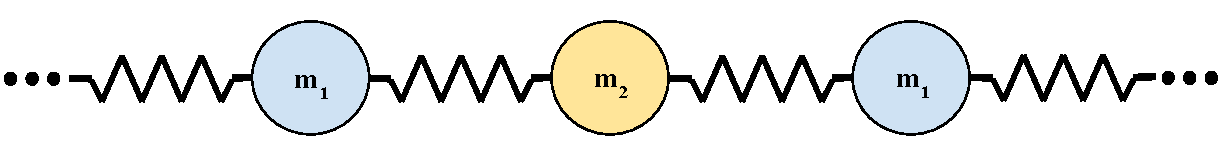
\includegraphics[width=0.75\textwidth]{diatomic-mass-spring.pdf}
	\caption{A system of alternating masses connected by springs extending 
	infinitely to the left and right.}
	\label{fig:dms}
\end{figure}

After assuming a harmonic motion
\begin{equation}
u_n = \tilde{u}(x_n)e^{i\omega t}
\end{equation}
The equations of motion for a diatomic lattice can be written
\begin{equation}
(-\omega^2m_2 + 2k)u_{2n} - k(u_{2n-1} + u_{2n+1}) = 0
\end{equation}
\begin{equation}
(-\omega^2m_1 + 2k)u_{2n+1} - k(u_{2n} + u_{2n+2}) = 0
\end{equation}
We can write this in a matrix for
\begin{equation}
(\mathbf{K}_n - \omega^2 \mathbf{M})\mathbf{u}_n + 
\mathbf{K}_{n-1}\mathbf{u}_{n-1}
+ \mathbf{K}_{n+1}\mathbf{u}_{n+1} = 0
\end{equation}
where
\begin{equation}
\mathbf{u}_n =
\begin{bmatrix}
u_{2n} \\
u_{2n+1}
\end{bmatrix}
\end{equation}

We will use the inverse method to solve for the dispersion relation. We use 
Bloch's theorem to write
\begin{equation}
\mathbf{u_n}= \mathbf{\hat{u}}(\mu)e^{in\mu}
\end{equation}

Finally, we can write
\begin{equation}
\left[\mathbf{K}_n + \mathbf{K}_{n-1}e^{-i\mu} + \mathbf{K}_{n+1}e^{i\mu} 
-\omega^2 \mathbf{M} \right] \mathbf{\hat{u}}(\mu)e^{in\mu} = 0
\end{equation}

\begin{equation}
\left[\mathbf{\Bar{K}}(\mu) -\omega^2 \mathbf{M} \right] 
\mathbf{\hat{u}}(\mu)e^{in\mu} = 0
\end{equation}

Calculating the determinant of the matrix on the left we get the relation
\begin{equation}
\omega =\pm \sqrt{k\frac{m_1+m_2}{m_1m_2} \pm k 
\sqrt{\left(\frac{m_1+m_2}{m_1m_2}\right) - \frac{4(\sin{ka})^2}{m_1m_2}}}
\end{equation}

\subsubsection{Transfer matrix method}
The transfer matrix method enforces continuity between layers of a system. At 
the interface between two unit cells the displacements must be equal and the 
forces or tractions must be as well. First, a relationship between these 
variables must be derived from one end of the unit cell to the other end. This 
results in the formulation of a so called transfer matrix. This type of 
analysis is completed by of course applying Bloch's theorem to relate the 
displacements and forces in one cell to another.

%----------------- COMPUTATIONAL METHODS FOR PHONONIC MEDIA -------------------%
%  We jut got done talking a lot about dispersion relations. To make this jump
%  Computational methods we need make a point about how for nontrivial systems
%  and continuum systems that sort of analysis isn't as realistic
%  also talk about why we are specializing in finite elements. When you get to
%  finite elements explain what is actually happening in the code for people
%  who aren't as familiar with these computational methods
%------------------------------------------------------------------------------%
\section{Computational methods for phononic media} \label{methods}
\subsection{Plane-wave expansion method}
According to \cite{cao04}, the plane-wave method is widely used because of its 
convenience. Apparently, the drawback of the method is slow convergence.
\begin{enumerate}
	\item To start expand the displacements and material properties in the wave 
	equation in terms of a Fourier series (assert solutions in the form of 
	Bloch waves)
	\item Substitute these expansions back into the wave equation
	\item After forming some kind of inner products, an eigenvalue problem can 
	be found
	\item In order to actually find the dispersion relations, one must solve 
	the eigenvalue problem for a range of wave numbers
\end{enumerate}

\subsection{Finite difference method}
Finite difference methods are similar to the plane wave expansion method with 
the advantage that the solution convergence is faster for materials with 
multiple phases
\begin{enumerate}
	\item Instead of expanding the solution on material properties, the 
	differential operators of the wave equation are expanded using standard 
	finite differences
	\item The equations of motion can be written as a matrix equation
	\item An eigenvalue problem appears after asserting a Bloch wave type 
	solution
	\item Once again the eigenvalue problem must be solved for a range of wave 
	numbers
\end{enumerate}

\subsection{Finite element method}
The finite element method is useful for complex material geometries. When 
applied to periodic systems, the domain of computation is greatly reduced via 
application of Bloch's theorem. The standard outline for the finite element 
method is as follows
\begin{enumerate}
	\item Formulate the weak form of the wave function by multiplying by a 
	trial function and integrating
	\item Write the equation in matrix form by allowing the solution to be 
	expressed as a combination of weight functions
	\item Apply the Bloch's theorem
	\item Solve the resulting eigenvalue problem for a range of wave numbers
\end{enumerate}

\subsection{Multiple scattering method}
Compared to the above methods, the multiple scattering method has an advantage 
when the material under consideration contains scattering elements 
(resonators?). The method relies on separating the solution into fields 
associated with the incident wave and then waves scattered from each scattering 
element in the system. Once the solution, at a single scattering element a 
system of equations can be solved for the rest of the scattered fields. The 
dispersion relations are then found by application of Bloch's theorem. 

%---------- ANALYSIS OF LATTICE STRUCTURES VIA REAL TIME EVOLUTION ------------%
%  Real time evolution is sort of like a finite difference method right? But it 
%  is not the finite difference scheme described above. You are going to have 
%  frame this correctly so that the audience knows why this type of analysis 
%  is useful. Really, how does looking at the real time evolution fit the 
%  story you are trying to tell about dispersion relations and and this whole 
%  thing with Bloch's theorem
%------------------------------------------------------------------------------%
\section{Analysis of lattice structures via real time evolution}

\subsection{Monatomic lattice}
Here we verify the results of Section \ref{monatomic}. The system is modeled 
using the equations of motion (\ref{eqnms}) and the Verlet integration method. 
Figure \ref{fig:matlab-dr} displays the dispersion relation for the mass spring 
system which has been calculated from the real time evolution of the system. 
The system is excited in a range of frequencies between $\Omega=0$ and 
$\Omega=2$. For each of the frequencies, the system is allowed to evolve and 
the Fourier transform of the resulting wave is computed. In the reciprocal 
space, there is an obvious peak at one wave number. This wave number is then 
plotted with its corresponding frequency.
\begin{figure}[!htbp]
	\centering
	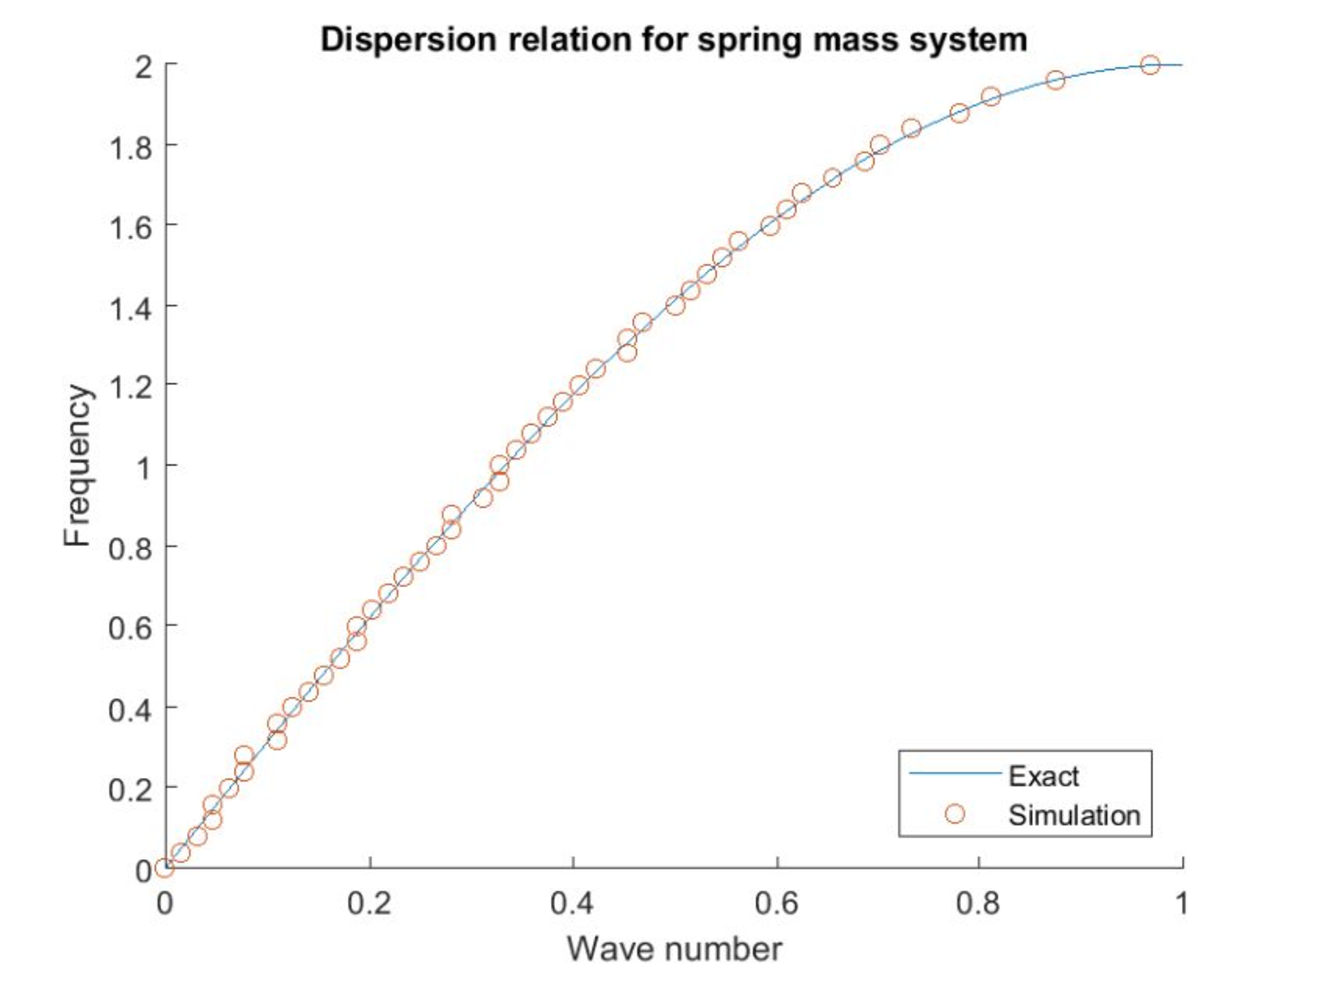
\includegraphics[width=0.75\textwidth]{matlab-dr.pdf}
	\caption{Using a Fourier transform in space, wave lengths for different 
	excitation frequencies are identified and plotted}
	\label{fig:matlab-dr}
\end{figure}

Applying a sinusoidal, forcing term to the first mass it is easy to explore the 
attenuation effect at the stop band as seen in Figure \ref{fig:dr}. Figures 
\ref{fig:snap19} and \ref{fig:snap21} display snapshots of the system at 
excitation frequencies above and below $\Omega=2$. There is an obvious drop in 
amplitude inside and outside of the stop band.
\begin{figure}[!htbp]
	\centering
	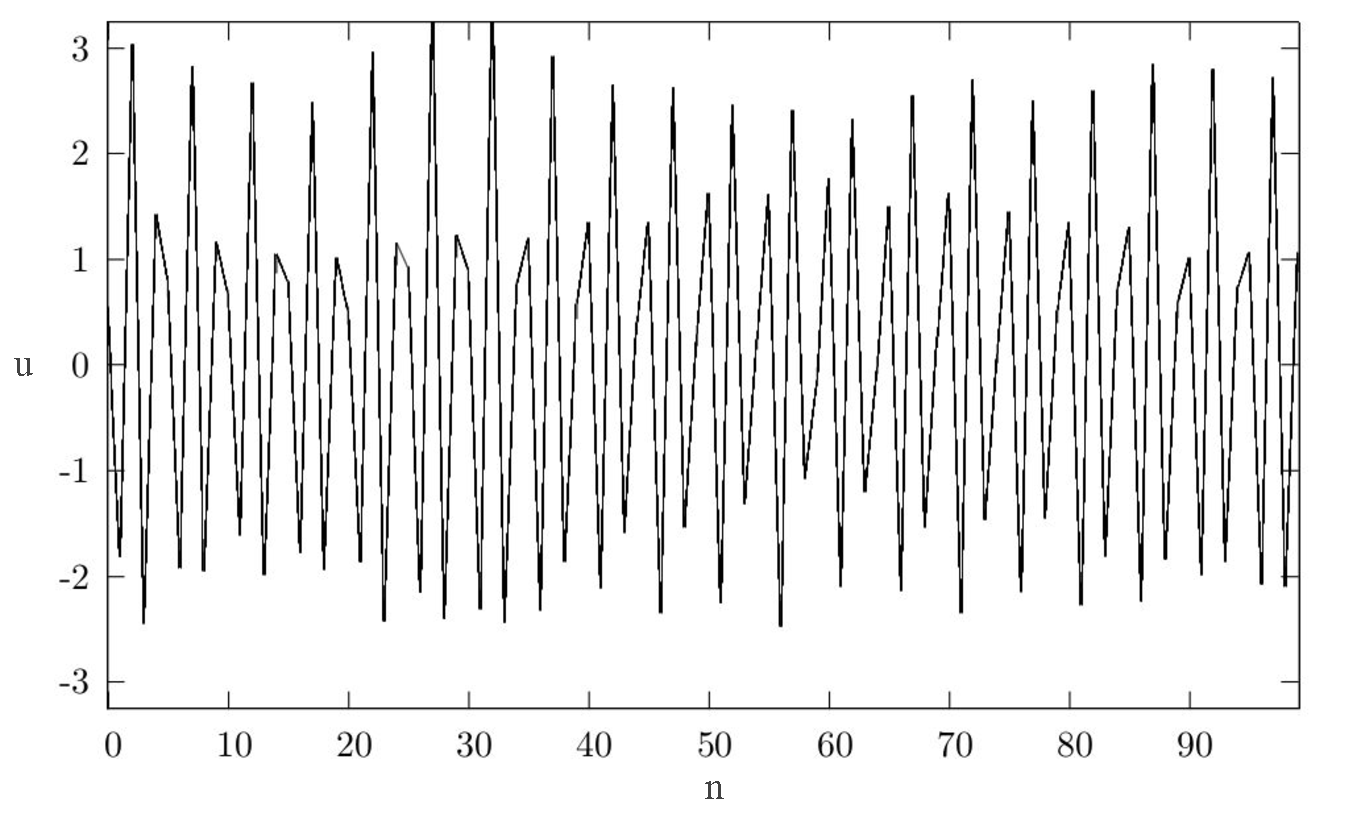
\includegraphics[width=0.75\textwidth]{snap-f19.pdf}
	\caption{Snapshot of mass spring system with $\Omega=1.9$}
	\label{fig:snap19}
\end{figure}
\begin{figure}[!htbp]
	\centering
	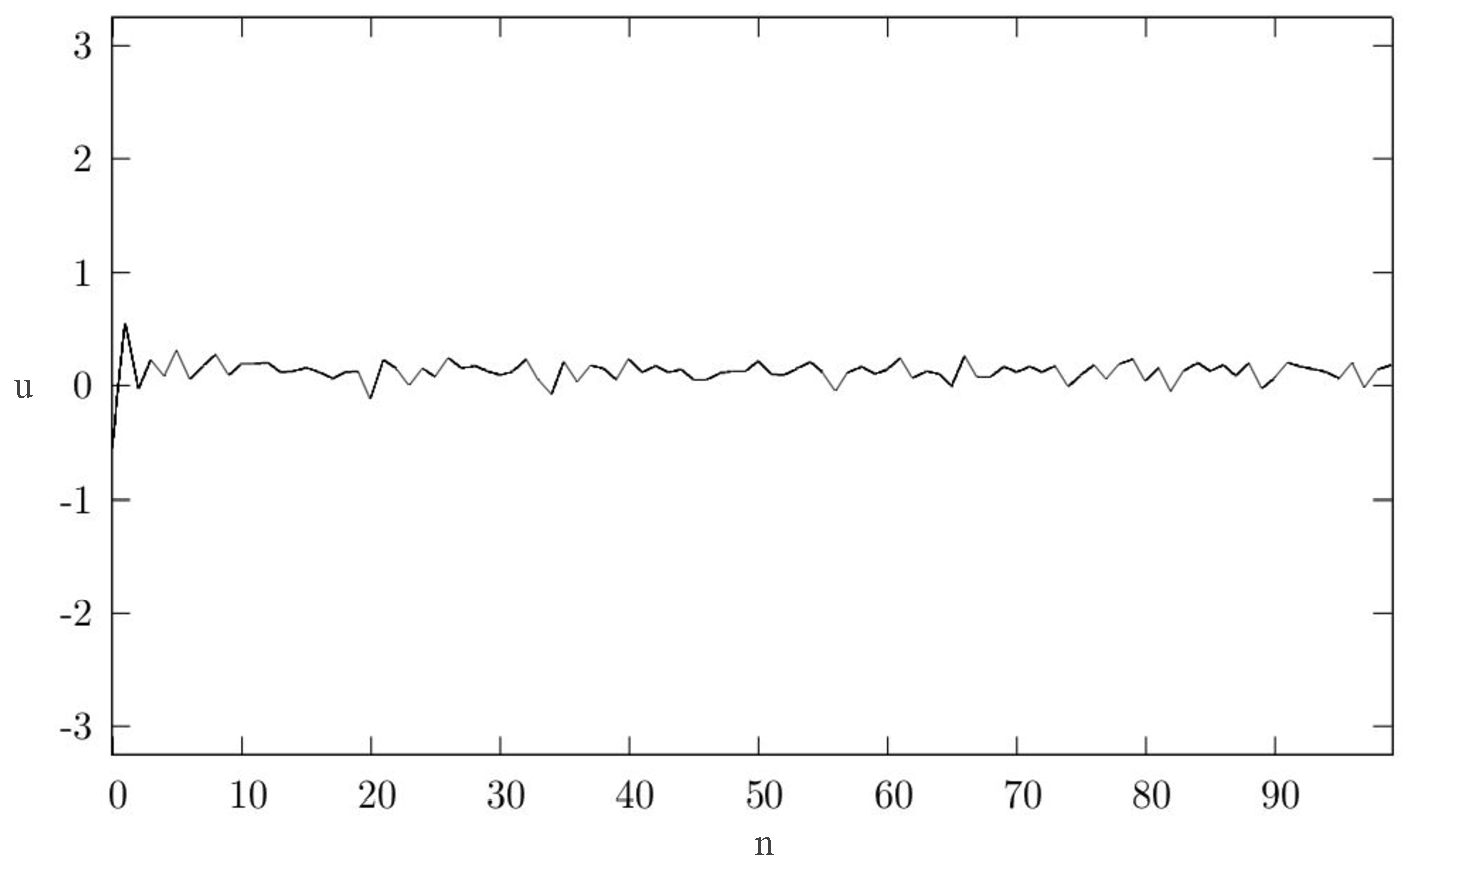
\includegraphics[width=0.75\textwidth]{snap-f21.pdf}
	\caption{Snapshot of mass spring system with $\Omega=2.1$}
	\label{fig:snap21}
\end{figure}

\subsection{Diatomic lattice}
Here the results for a diatomic lattice are presented from a similar simulation 
to the above.
\begin{figure}[!htbp]
	\centering
	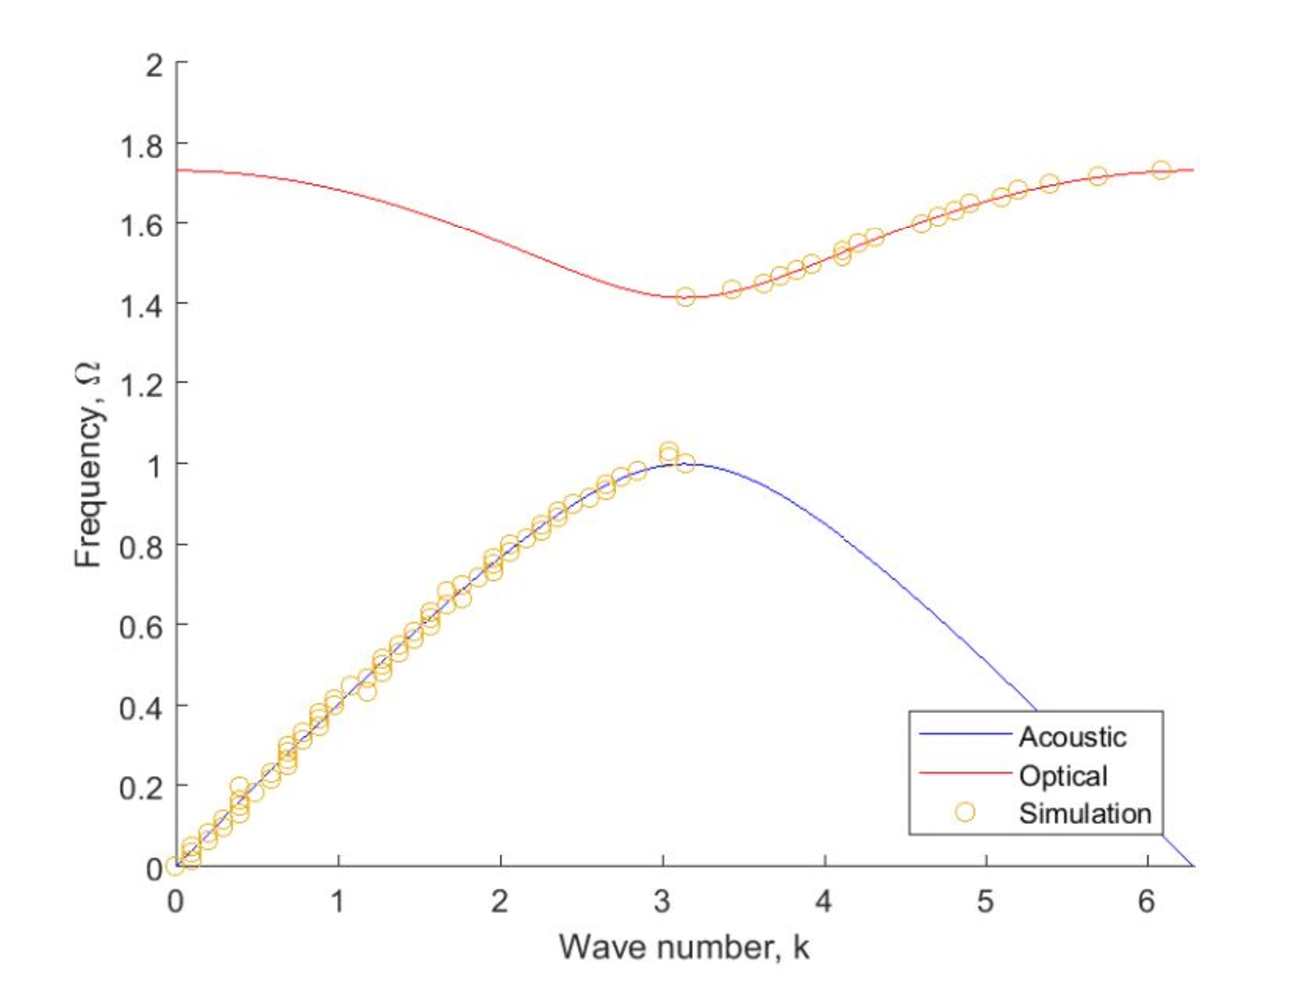
\includegraphics[width=0.75\textwidth]{diatomic-dr.pdf}
	\caption{Dispersion relation for the diatomic lattice}
	\label{fig:diadr}
\end{figure}

%------ ANALYSIS OF 1D CONTINUUM MATERIALS VIA FINITE ELEMENT METHOD ----------%
%  Here is where you connect with Bloch's theorem and what is a powerful method 
%  of analysis that will be used in actual research. Emphasize the importance 
%%%  of this and its utility.
%------------------------------------------------------------------------------%
\section{Analysis of 1D continuum materials via finite element method}
\subsection{Uniform bar}
As a first exercise in using finite elements to find the dispersion properties 
of materials, we will solve for the real time evolution of a waves in a bar and 
find the dispersion relation in a similar manner as in the mass-spring system 
(using the Fourier transform in space). For the one dimensional problem, the 
elasticity equations we want to solve are.
\begin{align}
\frac{\partial \sigma_x}{\partial x} + b_i &= \rho \frac{\partial^2 
u_x}{\partial t^2},\quad x\in[0,L]\quad\textnormal{(Equilibrium)} \\
\sigma_x &= E \varepsilon_x\quad\textnormal{(Constitutive relation)}\\
\varepsilon_x &= \frac{\partial u_x}{\partial 
x}\quad\textnormal{(Strain-displacement)}\\
u_x(x=0,t) &= A_0sin(\omega t) \\
\sigma_x(x=L,t) &= 0
\end{align}
Note that the finite element solution with $n$ nodes is analogous to the mass 
spring system with $n$ masses. Here, we can relate the material properties via 
$\rho = \frac{M}{AL}$ and $E = \frac{kL}{A}$. Thus, for a system of n masses, 
the analogous system in finite elements has material properties
\begin{equation}
\rho = \frac{n}{d(n-1)}
\end{equation}
and
\begin{equation}
E = \frac{k_{eff}\times d(n-1)}{1}= (1/k +\cdots)^{-1} \times d(n-1)= 
\frac{d(n-1)}{n}
\end{equation}
where $L=d(n-1)$ and we require that the nodes have the spacing with respect to 
each other as the springs to with each other.

In the absence of body forces, we can find the weak form of the equilibrium 
equation by multiplying by a test function $\varphi$ and integrating of the 
domain.
\begin{equation}
\int_0^L \varphi \frac{\partial \sigma_x}{\partial x} dx
= \int_0^L \varphi \rho \frac{\partial^2 u_x}{\partial t^2} dx
\end{equation}
Using integration by parts on the LHS of the above we find that
\begin{equation}
\varphi(L)\sigma_x(L) - \varphi(0)\sigma_x(0) 
- \int_0^1 \frac{\partial \varphi}{\partial x} \sigma_x dx
= \int_0^L \varphi \rho \frac{\partial^2 u_x}{\partial t^2} dx
\end{equation}
Applying boundary conditions, constitutive relation, and the 
strain-displacement equation we arrive at the weak form of the equation
\begin{equation}
\int_0^1 \frac{\partial \varphi}{\partial x} E \frac{\partial u_x}{\partial x} 
dx
+ \int_0^L \varphi \rho \frac{\partial^2 u_x}{\partial t^2} dx = 0
\end{equation}
Now, we approximate our test function and solution using linear shape functions
\begin{align}
\varphi &= N_i(x) \\
u_x &= \sum_j a_j(t)N_j(x)
\end{align}
Then,
\begin{equation}
\int_0^1 \frac{\partial N_i(x)}{\partial x} E \sum_j\frac{\partial 
N_j(x)}{\partial x} a_j dx
+ \int_0^L N_i \rho \sum_j N_j \frac{\partial^2 a_j(t)}{\partial t^2} dx = 0
\end{equation}
Rearranging,
\begin{equation}
\int_0^1  E \sum_j\frac{\partial N_i(x)}{\partial x}\frac{\partial 
N_j(x)}{\partial x} a_j dx
+ \int_0^L \rho \sum_j  N_i N_j \frac{\partial^2 a_j(t)}{\partial t^2} dx = 0
\end{equation}
Finally, we write the above equation in matrix form
\begin{equation} \label{matrixform}
Ka+M\ddot{a} = 0 
\end{equation}
where $K$ is called the stiffness matrix, and $M$ is called the mass matrix. 

We now assume a solution of the form
\begin{equation}
a = ae^{i(kx-\omega t)}
\end{equation}
such that the second order differential equation (\ref{matrixform}) becomes a 
complex eigenvalue problem:
\begin{equation}
Ka - \omega^2 Ma = (K-\omega^2M)a = 0
\end{equation}
Note that as of now $K$ and $M$ are not functions of the wave number and 
solving the eigenvalue problem as is does not yield any information about the 
dispersion properties of the system. To obtain this dependence the Bloch 
condition must be enforced. 

The Bloch condition is similar to the periodic boundary condition
\begin{equation}
a(x+h) = a(x)\quad\textnormal{(Periodic boundary condition)}
\end{equation}
where h is the size of the unit cell. The difference between the two conditions 
is a single multiplicative factor:
\begin{equation}
a(x+h) = e^{ik_xh}a(x)\quad\textnormal{(Bloch condition)}
\end{equation}
The multiplicative factor in the boundary condition shifts is such that when 
the wave reaches a boundary it is phase shifted to match the wave at the 
opposite boundary such that there is no interference.

Enforcing the condition is done via a linear transformation which in one 
dimension is
\begin{equation}
T = 
\begin{bmatrix}
1 && \mathbf{0} \\
\mathbf{0} && \mathbf{I}\\
e^{ik_xh} && \mathbf{0}
\end{bmatrix}
\end{equation}
where $\mathbf{I}$ is an identity matrix with dimensions equal to the number of 
interior nodes (in the one dimensional case this is the total number of nodes 
minus two). Using this transformation matrix we reduce the number of degrees of 
freedoms in our system and write
\begin{equation}
a =
\begin{bmatrix}
a_{left} \\
a_{int} \\
a_{right}
\end{bmatrix}
= 
\begin{bmatrix}
1 && \mathbf{0} \\
\mathbf{0} && \mathbf{I}\\
e^{ik_xh} && \mathbf{0}
\end{bmatrix}
\begin{bmatrix}
a_{left} \\
a_{int}
\end{bmatrix}
= T \hat{a}
\end{equation}
Our eigenvalue problem is now
\begin{equation}
(K-\omega^2M)T\hat{a} = 0
\end{equation}
To make it so our matrix is square, and therefore invertible, we premultiply 
the equation by $T^T$
\begin{equation} \label{evalprob}
(\hat{K} - \omega^2 \hat{M})\hat{a} = 0
\end{equation}
where
\begin{equation}
\hat{K}(k_x) = T^T K T
\end{equation}
and 
\begin{equation}
\hat{M}(k_x) = T^T M T
\end{equation}
We are now in position to extract the dispersion properties of the uniform bar. 
The eigenvalue problem is solved several times for values of $k_x$, and we 
obtain several corresponding values for $\omega$. 

\subsection{Layered composite}

%------ ANALYSIS OF 2D CONTINUUM MATERIALS VIA FINITE ELEMENT METHOD ----------%
%  At this point you have already explained what finite elements is in 1D. You
%  will need to reiterate the process but explain in detail the new equations 
%  for 2D finite elements. Additionally, what new sorts of phenomena do we 
%  expect to see here. What are the difficulties? What are the new
%  consideration? What are the new results? etc.
%------------------------------------------------------------------------------%
\section{Analysis of 2D continuum materials via finite element method}

\subsection{Uniform material}

\subsection{Laminate}

\subsection{Material with inclusions}

%------------------------------- FUTURE WORK  ---------------------------------%
%  This one will be a little difficult. Assuming you have done your literature 
%  review correctly, you should be in a position to speak about the direction 
%  you will take. This is where you take ownership of this project. Be sure to 
%  Connect with the methods of analysis you have been talking about here, but
%  also to the beginning of this report where you have outlines the frontiers
%  of research in phononic media.
%------------------------------------------------------------------------------%
\section{Future work}

%-------------------------------- CONCLUSION  ---------------------------------%
%  Recapitulate and make sure that the audience knows that you are in a 
%  position to make contributions to the field. This part is important. Once 
%  again frame it so they know what has been done in the field and what hasn't.
%  The things you need to do what hasn't been done and how you have mastered 
%  them.
%------------------------------------------------------------------------------%
\section{Conclusion}

%------------- ADDITIONAL STUDIES OF HETEROGENEOUS MATERIALS  -----------------%
%  Here quickly outline the chapters of the lecture notes that you studied and 
%  some of the techniques that you have learned. Much like the proposal for 
%  this independent study
%------------------------------------------------------------------------------%
\section{Additional studies of heterogeneous materials}
In addition to this study of phononic media, much time and effort was put into 
the notes of Prof. Ponte-Casta\~neda. Attached to this document, are solutions 
to various problems in the lecture notes. 

\section{Acknowledgements}
I would like to thank my advisors Prof. Ponte-Casta\~neda and Prof. Reina for
guidance this semester. Additionally, I would like to thank Chenchen Liu of
Prof. Reina's group for helping me get a grip of using finite elements and Bloch
analysis for this phononic media.

\appendix
\section{Appendix}
\subsection{Verlet integration}
For a single particle, the Verlet integration method is used to calculate its 
trajectory given that the forces (and therefore the acceleration) are known. 
The algorithm is
\begin{equation}
x^{t+1}_{n} = 2x^{t}_{n} - x^{t-1}_{n} + a(x^{t}_n)\Delta t^2
\end{equation}
where $t$ denotes the current time step, $x$ is the particle position, $a(x_n)$ 
is the acceleration, and $\Delta t$ is suitably small time step. b

\subsection{Finite difference in time for real time evolution FEM}
For equation (\ref{matrixform}), it is possible to apply a finite difference 
method in time in order to get the real time evolution of the uniform bar. 
First, in order to apply the displacement boundary conditions at the left 
boundary, we need to modify (\ref{matrixform}). We partition the matrices 
\begin{equation} \label{partition}
\begin{bmatrix}
K_{11} & K_{1a} \\
K_{a1} & K_{aa}
\end{bmatrix}
\begin{bmatrix}
a_1 \\
a
\end{bmatrix}
+
\begin{bmatrix}
M_{11} & M_{1a} \\
M_{a1} & M_{aa}
\end{bmatrix}
\begin{bmatrix}
\ddot{a_1} \\
\ddot{a}
\end{bmatrix}
= 0
\end{equation}
Here, $K_{11}$ and $M_{11}$ denote the entry in the first row and first column. 
$K_{1a}$ and $M_{1a}$ are row vectors of the rest of the entries in the first 
row and $K_{a1}$ and $M_{a1}$ are column vectors of the remaining elements of 
the first column. $K_{aa}$ and $M_{aa}$ are then matrices of the remaining 
elements of the matrices $K$ and $M$. Since we know $a_1$ and $\ddot{a_1}$ 
(these are the displacement and acceleration at the first node), we only wish 
to solve the bottom row of ($\ref{partition}$).
\begin{equation}
K_{aa}a + M_{aa}\ddot{a} = -a_1K_{a1} - \ddot{a_1}M_{a1}
\end{equation}

To solve the above we discretize $\ddot{a}$ in time using an explicit finite 
difference scheme.
\begin{equation}
K_{aa}a^t + M_{aa}\frac{a^{t+1} - 2a^t + a^{t-1}}{\Delta t^2 } = 
-a_1^{t+1}K_{a1} - \ddot{a_1}^{t+1}M_{a1}
\end{equation}
Solving for $a^{t+1}$
\begin{equation}
a^{t+1} = M_{aa}^{-1}(-a_1^{t+1}K_{a1} - \ddot{a_1}^{t+1}M_{a1} - 
K_{aa}a^t)\Delta t^2 
+ 2a^t - a^{t-1}
\end{equation}

\bibliography{mybib}{}
\bibliographystyle{unsrt}

\end{document}
